\newpage
\section{Aufbau und Durchführung}

\subsection{Aufbau}

\begin{figure}
    \begin{subfigure}{0.5\textwidth}
        \centering
        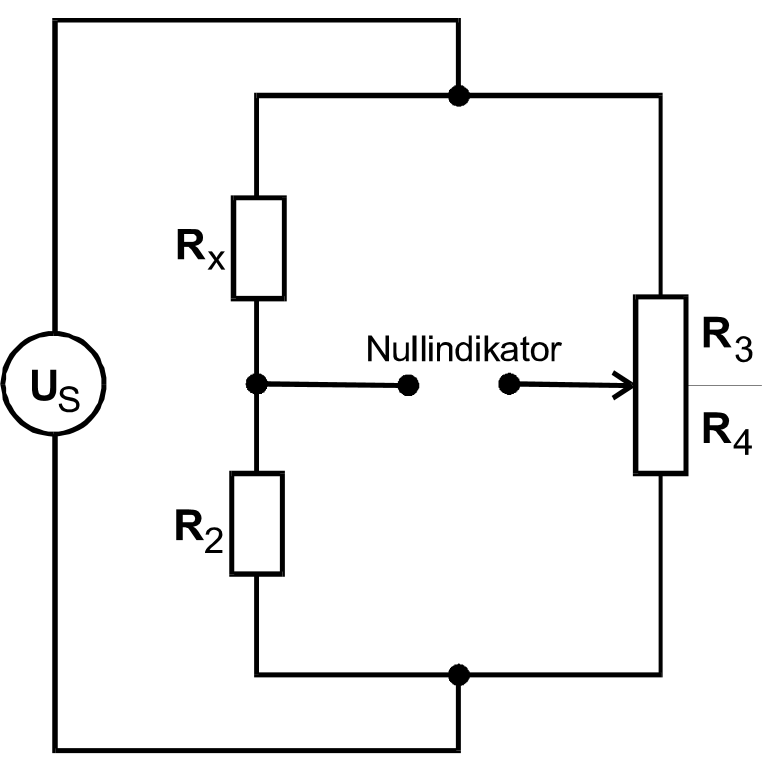
\includegraphics[height=4cm]{Bilder/Wheatstone.png}
        \caption{Wheatstonesche Brückenschaltung}
        \label{fig:Wheatstone}
    \end{subfigure}
    \begin{subfigure}{0.5\textwidth}
        \centering
        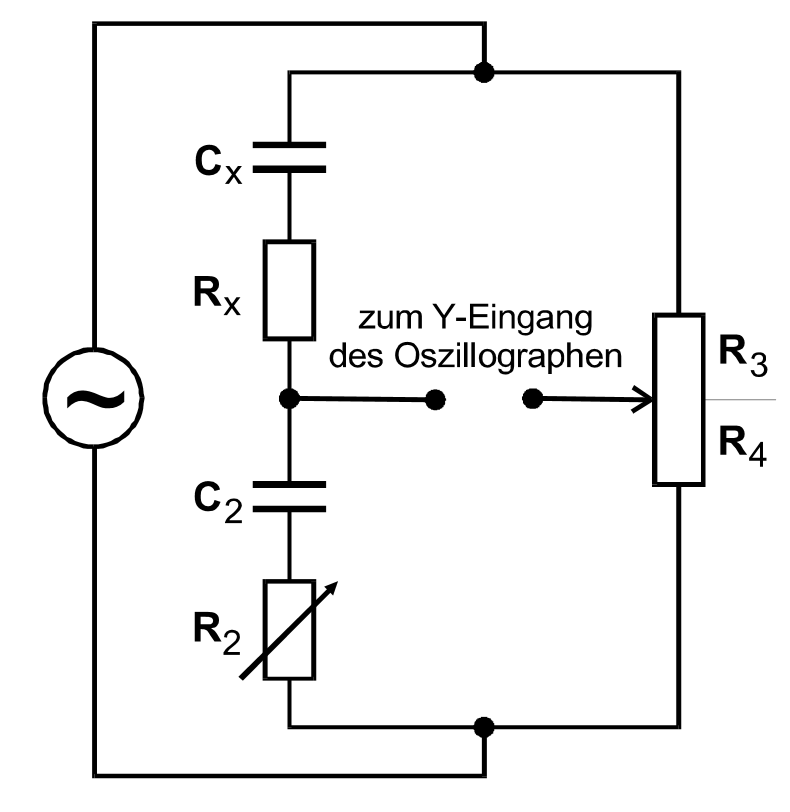
\includegraphics[height=4cm]{Bilder/Kapazitiv.png}
        \caption{Kapazitive Brückenschaltung}
        \label{fig:Kapazitiv}
    \end{subfigure}
    \begin{subfigure}{0.5\textwidth}
        \centering
        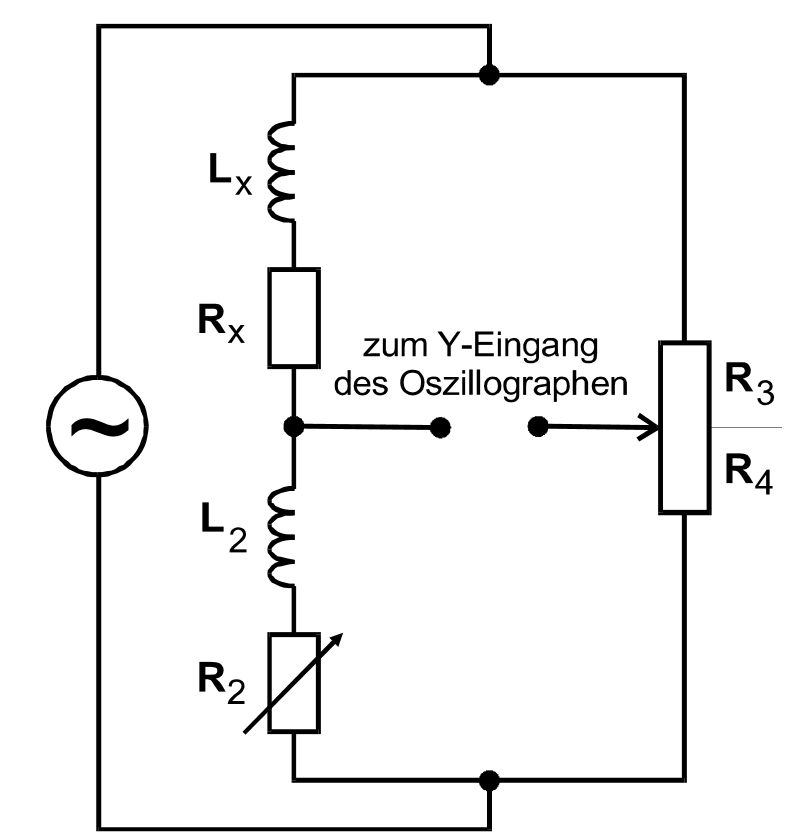
\includegraphics[height=4cm]{Bilder/Induktiv}
        \caption{Induktive Brückenschaltung}
        \label{fig:Induktiv}
    \end{subfigure}
    \begin{subfigure}{0.5\textwidth}
        \centering
        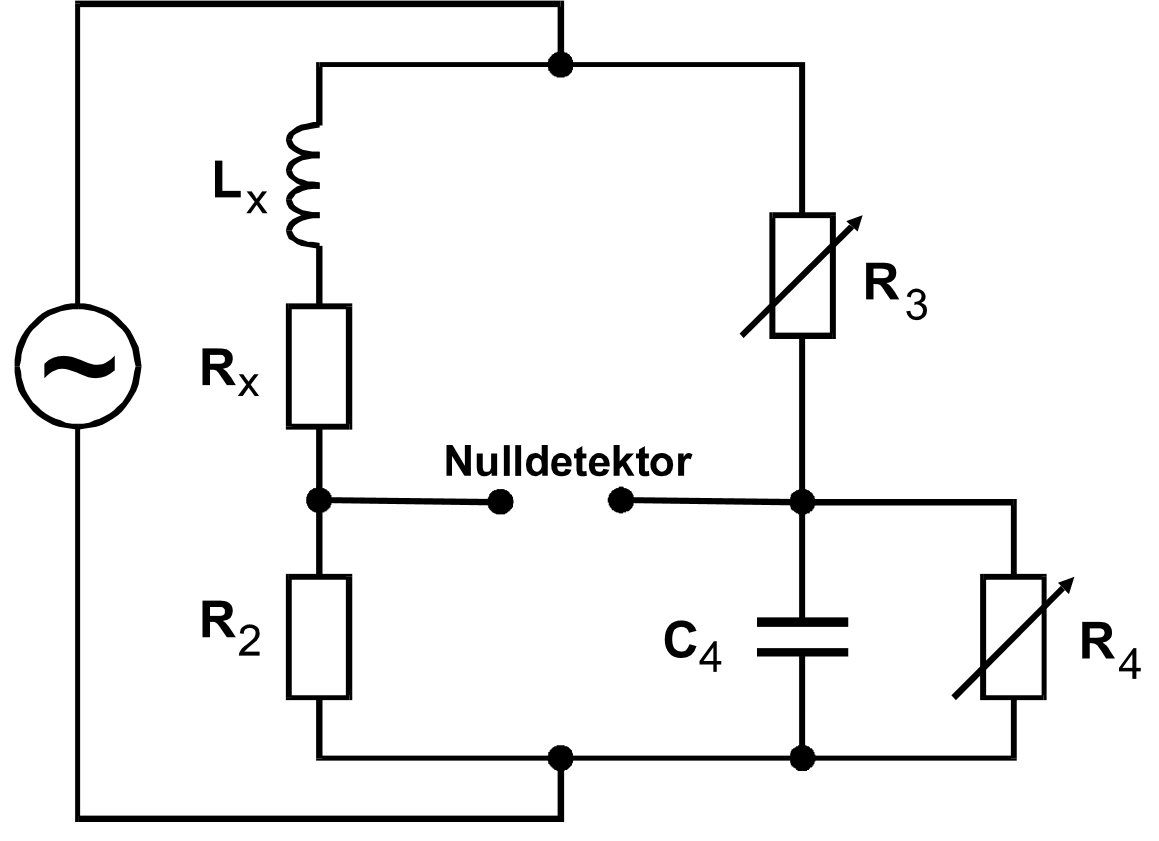
\includegraphics[height=4cm]{Bilder/Maxwell}
        \caption{Maxwellsche Brückenschaltung}
        \label{fig:Maxwell}
    \end{subfigure}
    \begin{subfigure}{0.5\textwidth}
        \centering
        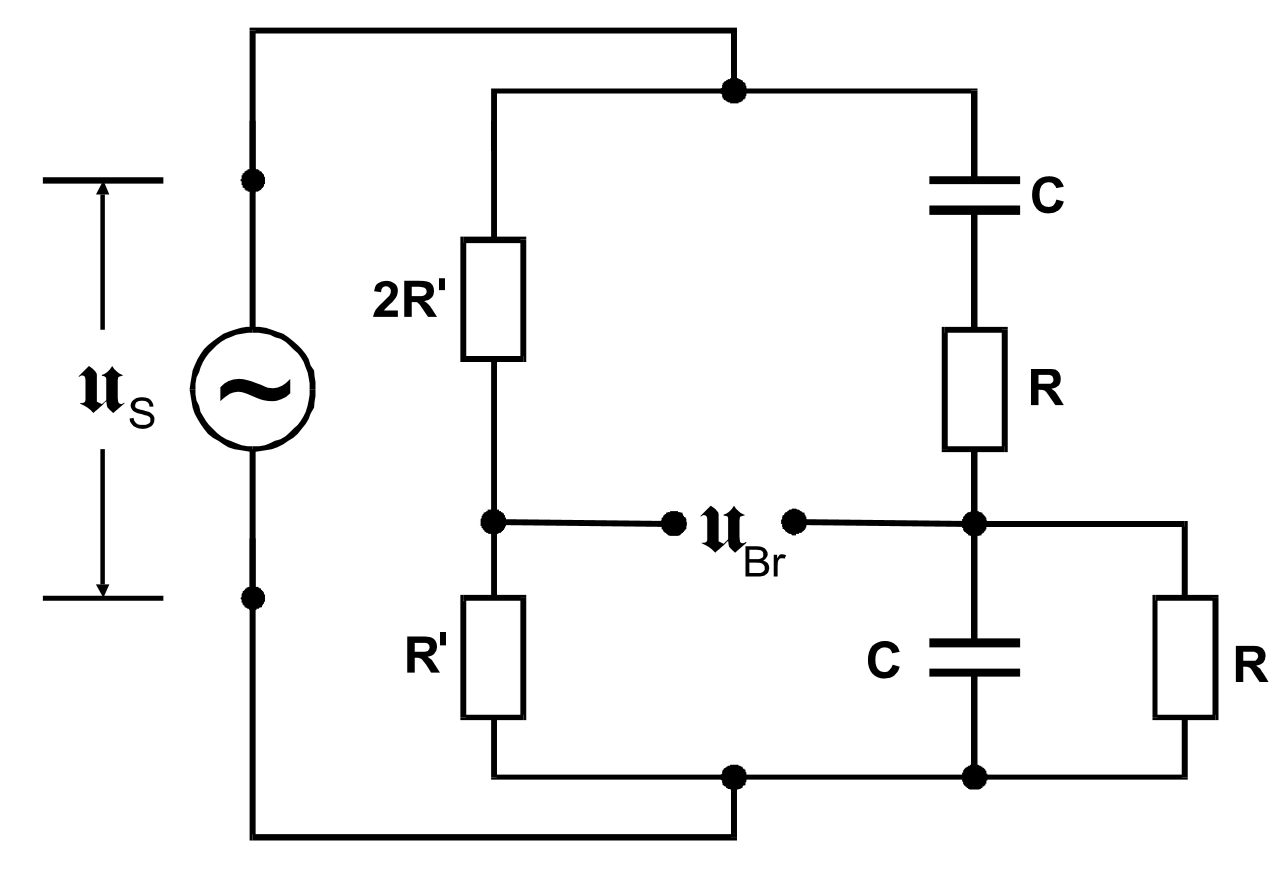
\includegraphics[height=4cm]{Bilder/Wien-Robinson}
        \caption{Wien-Robinson Brückenschaltung}
        \label{fig:Wien}
    \end{subfigure}
\end{figure}

\noindent Die Schaltkreise, entsrechend der Schaltbilder, werden%fehlende Referenz (Formulierung nochmal überlegen)
mit vorgefertigten Bauteilen zusammengefügt, wobei bestimmte Elemente unbekannte Werte haben.
Als Spannungsmessgerät wird ein Oszilloskop verwendet. $R_3$ und $R_4$ sind Potentiometer, wobei für
für die ersten drei Schaltungen gilt, dass $R_3+R_4=\qty{1000}{\ohm}$ ist.

\subsection{Durchführung}

In der Wheatstoneschen Brückenschaltung (\ref{fig:Wheatstone}) müssen $R_3$ und $R_4$ variiert werden, 
bis im Oszilloskop die Brückenspannung auf $\qty{0}{\volt}$ fällt.

Bei der Kapazitiven, der Induktiven und der Maxwellschen Brückenschaltung hingegen wird durch Überlagerungen
der Grundschwingung der Wechselspannung mit Oberschwingungen gestört. Also wird nur ein Spannungsminimum 
durch das Variieren der ohmschen Widerstände erreicht.

Mit der Wien-Robinson Schaltung werden nun nur Bauteile mit bekannten Größen gewählt und die Frequenz $f$ 
der Eingangsspannung geändert. Zu jeder betrachteten Frequenz wird dann die Brückenspannung aufgetragen.



\label{sec:Durchführung}
